\section{Methods}
\label{sec:methods}

Figure \ref{system} provides an overview of the steps taken in the proposed methodology for predicting fatigue levels of sport horses during exercise.

\begin{figure}[htb]
\centering
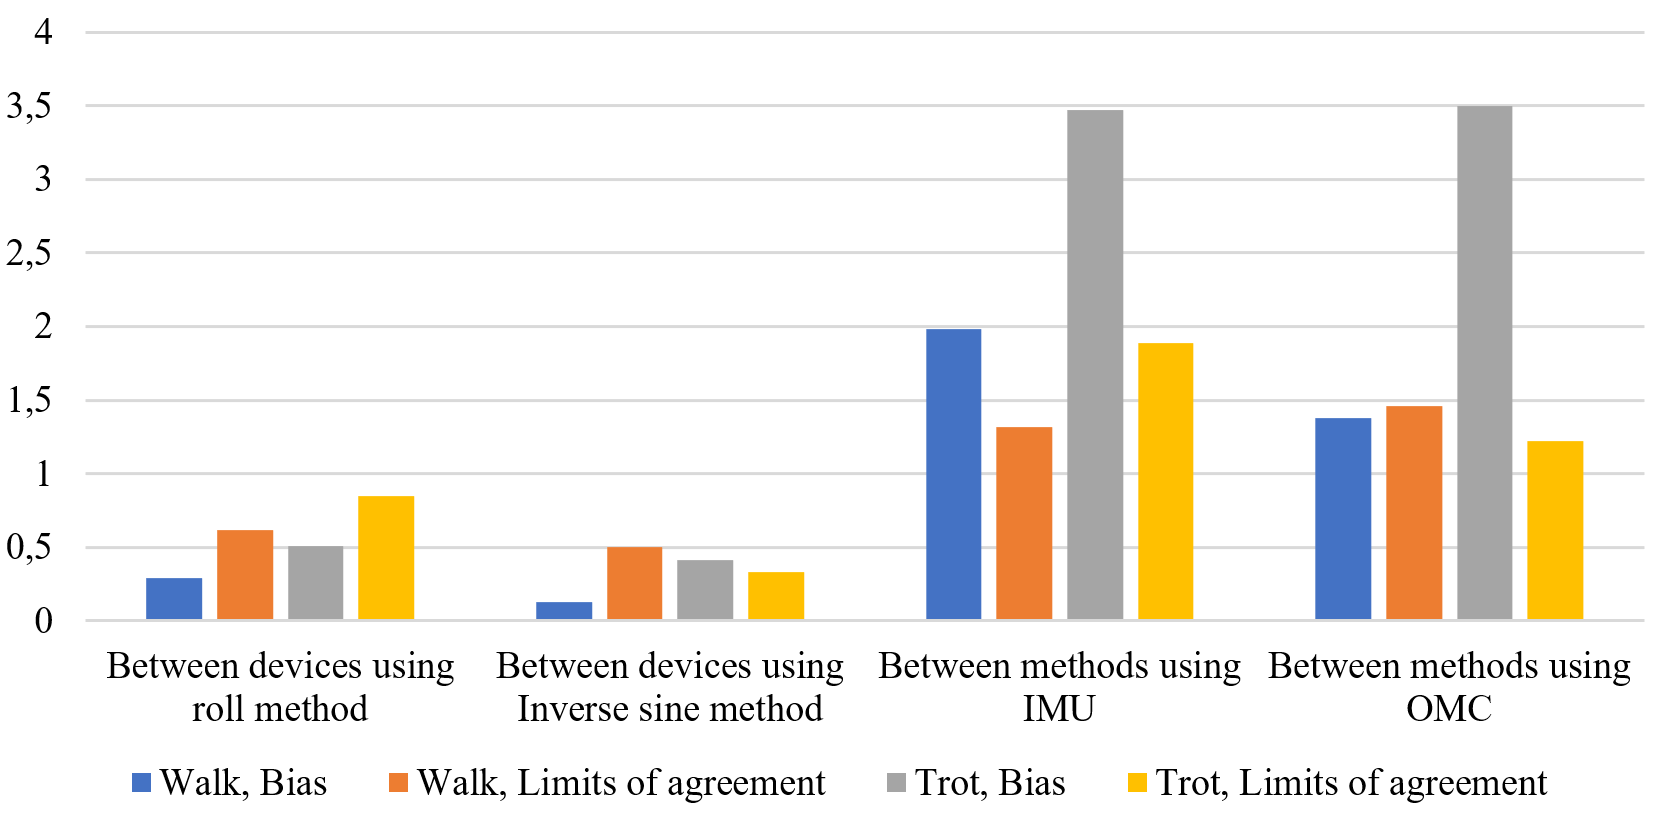
\includegraphics[width=0.95\linewidth]{chapters/fatigue/figures/Picture1.png}
\caption{An overview of the proposed method.}
\label{system}
\end{figure}

\subsection{Data preparation}
In chapter \ref{chapter:data}, the details of the data collection procedure were described thoroughly. For this chapter, we selected the data from eventing horses. The SETs (for the SET protocol refer to chapter \ref{sec:trainingprotocol}) were collected with the sacrum, withers, and right front limb IMUs, however, we excluded the withers \gls{imu} and used only the two \gls{imu}s that were mounted on the sacrum and right front limb (Figure \ref{imuplacementsporthorse}). The exclusion helped us to include more horses in the study since some of the horses lacked the withers \gls{imu} data as was shown earlier in Table \ref{tab:IMU info on horses}. Throughout the rest of this chapter, we will use the term "limb" to specifically denote the right front limb. The \gls{lac} values from the \gls{set} of the eventing horses are demonstrated in Figure \ref{lactate_heat_map}.

\begin{figure}[htb]
\centering
\includegraphics[width=.95\linewidth]{chapters/fatigue/figures/Picture2.png}
\caption{\gls{lac} values of participants. The 5th \gls{lac} values of participants 1, 4, 6, 7, and 14 are empty (indicated by a white color) due to reaching 4 \gls{mmol/L} in their 4th \gls{lac} values.}
\label{lactate_heat_map}
\end{figure}

%\subsection{Dataset preparation}
The collected data from the \gls{imu}s, the \gls{hr} monitor, and plasma \gls{lac} measurements were time-synchronized. All six acceleration and angular velocity signals were used from the sacrum \gls{imu}, while only the three angular velocity signals from the limb \gls{imu} were used. The acceleration signals from limb \gls{imu} were excluded due to the high training intensity, which caused the acceleration values to surpass the ±8g threshold of the \gls{imu}'s initial settings.

The extracted signals from \gls{imu}s were smoothed using a Savitzky-Golay polynomial filter \cite{Karaim2019-gh}. Since there is at least one cantering stride within one second, the filtered signals were windowed into windows wider than one second to cover at least one full stride. To find the impact of different window sizes on the model performance, we chose two, four, and eight-second windows (400, 800, and 1600 samples). Consecutive windows were extracted from the signals by applying a sliding step of 75 percent of the window size (or 25 percent overlap). 

\subsection{Lactate Accumulation Calculation}
As mentioned, only six \gls{lac} value was collected for each horse during \gls{set}. However, a more extensive dataset was required for developing a model to estimate \gls{lac}. As a solution, we converted the discrete \gls{lac} measurements into continuous data. In the existing literature, a relationship has been established between \gls{lac} and \gls{hr} \cite{Munsters2020AStudy,Manzi2009-xy},

\begin{equation}y=be^{cx}\end{equation}

This formula is participant-dependent and derives from the $\Delta HR$-\gls{lac} response curve, where x is the fractional elevation of \gls{hr} (indicated as $\Delta HR$) and y is \gls{lac}. $\Delta HR$ comes from:

\begin{equation}\Delta HR=\dfrac{HR_{exercise}-HR_{rest}}{HR_{maximal}-HR_{rest}}\end{equation}

To fit the $\Delta HR$-\gls{lac} curve, a \gls{set} with increasing intensity is required. This is because elevating the SET intensity leads to higher LA and HR values, rendering it conducive to fitting an exponential curve to the data points plotted. Therefore, we excluded the first (at rest) and the sixth (after recovery) \gls{lac} samples (Figure \ref{lactate_heat_map}) from the $\Delta HR$-\gls{lac} plot, resulting in a maximum of four \gls{lac} samples per participant. Then, for each horse, the exponential curve was fitted to $\Delta HR$ and \gls{lac} datapoints, which could be four or fewer depending on the SET performed by the horse. An illustrative example of a fitted line in the $\Delta HR$-\gls{lac} plot for one of the participants is demonstrated in Figure \ref{deltahr_LA_plot}. Using the fitted curve, the individual-dependent factors, b and c, were extracted \cite{Munsters2020AStudy}. Using the formula and continuous $\Delta HR$ data from the \gls{set}, we calculated \gls{lac}, which we assigned as the generated \gls{lac} ($LA_g$). Finally, we combined $LA_g$ from all of the participants for the estimation model development. In order to assess $\Delta HR$, a resting heart rate of 30 \gls{bpm} and a maximum heart rate of 220 \gls{bpm} were employed \cite{Munsters2020AStudy} as the purpose of the SET was not measuring the maximum or the resting \gls{hr}. 


\begin{figure}[htb]
\centering
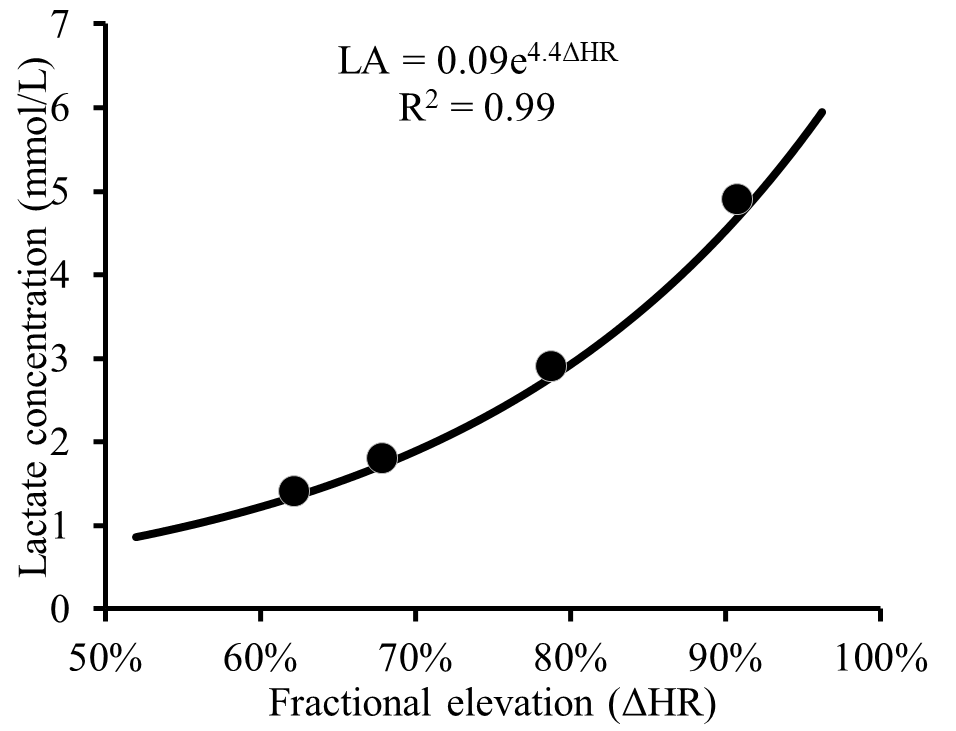
\includegraphics[width=.6\linewidth]{chapters/fatigue/figures/Picture4.png}
\caption{$LA_g$ plotted against the fractional elevation of \gls{hr} of a participant. The exponential line provides the calculation of the weighting factor (y).}
\label{deltahr_LA_plot}
\end{figure}


\subsection{Feature extraction}
\label{sec:subsets}

Feature extraction was implemented on the windows for the purpose of discovering the variables that significantly change the most by fatigue. The extracted features consisted of eleven signal-based features (per signal) and fifteen kinematics parameters (in total). 

The signal-based features, as presented in Table \ref{features_fatigue_chap}, serve as alternative representations of different signal aspects. For instance, the standard deviation was the most effective variability metric selected for sport horses fatigue classification, according to the results of chapter \ref{chapter:prepost}. Additionally, the foremost ranked feature in distinguishing the rider's impact on sport horses was the magnitude of the first coefficient obtained from the fast Fourier transform (FFT) of sacrum acceleration signal (Chapter \ref{chapter:rider}). Furthermore, regularity was computed by summing correlation coefficients aligned with peaks in the autocorrelation function of sacrum \gls{imu} vertical acceleration or limb \gls{imu} angular velocity \cite{Biau2004-mn}. Spectral energy sums up the squared magnitudes of all frequency components, providing a measure of the signal's energy distribution across different frequencies in the frequency domain. It's noteworthy that all frequency-related features were extracted from the FFT using the von Hann function to minimize spectral leakage and optimize outcomes \cite{smith1997scientist}.

\begin{table}[!htbp]
    \centering
    \caption{Signal-based and kinematic parameters}
    \resizebox{0.85\linewidth}{!}{% 
    \begin{tabular}{lccc}
    \toprule
        \textbf{Parameter description} & \multicolumn{3}{c}{\textbf{Extracted from}} \\ \cline{2-4}
        ~ & \textbf{Sacrum} & \textbf{Limb} & \textbf{Both} \\ \hline
        Signal-based features & ~ & ~ & ~ \\ \hline
        Maximum, Minimum, Mean, Median & 24 & 12 & 36 \\ \hline
        Standard deviation, First and third quartiles & 18 & 9 & 27 \\ \hline
        Detrended Fluctuation Analysis \cite{Bryce2012-jl} & 6 & 3 & 9 \\ \hline
        Spectral energy \cite{darbandi_2021_using}  & 6 & 3 & 9 \\ \hline
        Magnitude of the first three coefficients of FFT & 6 & 3 & 9 \\ \hline
        Stride regularity based on sacrum IMU \cite{Biau2004-mn} & 1 & - & 1 \\ \hline
        Stride regularity based on limb IMU & - & 1 & - \\ \hline
        Kinematic parameters & ~ & ~ & ~ \\ \hline
        Stride duration, stance, and swing duration, Speed & 4 & 4 & 8 \\ \hline
        Normalized Stride-Efficiency Factor (NSEF) & 1 & 1 & 2 \\ \hline
        Limb AROM & - & 3 & 3 \\ \hline
        Sacrum AROM and LROM, MaxDiff, MinDiff & 7 & - & 7 \\ \hline
        \textbf{Total} & \textbf{73} & \textbf{39} & \textbf{112} \\ \bottomrule
        
    \end{tabular}}
    \label{features_fatigue_chap}
\end{table}

In addition to the signal-based features, fifteen kinematic parameters were also calculated, as named in Table \ref{features_fatigue_chap}. These parameters were extensively discussed in previous chapters as vital parameters for evaluating equine health and fitness, and different methods were devised to calculate them using body-mounted \gls{imu}s.

Due to the \gls{set} protocol, both stride-related temporal parameters and speed increase inevitably throughout the \gls{set}, which might not reflect their true value. To have a normalized parameter that is not affected by the intensity and increment of the parameters, we define NSEF, which is calculated as:

\begin{equation}NSEF=\dfrac{\text{Stride duration}}{\text{Speed}}\end{equation}
	
The \gls{imu} signals were rigidly windowed, however, most of the kinematic parameters were based on a full stride. To address this, we utilized the stride event detection algorithm in chapter \ref{chapter:Step} to extract the maximum possible number of strides from each window, and subsequently calculated the kinematic parameters from the stride(s) within the window. In cases where more than one stride occurred within a window, we considered the average value of the kinematic parameters.



%\subsection{Data Normalization and Subsets}
To prepare the training and testing subsets, one of the horses was selected each time as the testing subset, and the remaining horses were assigned to the training subset. This process was repeated twenty-one times, ensuring that each of the horses was used exactly once as the testing subset. This approach allowed for comprehensive performance testing of the models with different combinations of horses in each fold. After each split, the features in the training subset were normalized using Z-score, as previously introduced in Equation \ref{eq:zscore}.

Which helps in improving the stability of machine learning models. Then, the testing set was normalized using the parameters from the training dataset normalization to remove the bias from the testing dataset. 

\subsection{Model training, testing and optimization}

Deep learning techniques were implemented on a selection of features or the training datasets as input and $LA_g$ as output. This has been done to assess the impact of \gls{hr} as a physiological feature on the model accuracy and to identify the compromised accuracy and improved performance on the single-\gls{imu} models due to fewer features. The training subsets were features from 1- \gls{hr} only, 2- \gls{hr} and both \gls{imu}s (\gls{imu}+\gls{hr}), 3- both \gls{imu}s (both-\gls{imu}s), 4- Sacrum \gls{imu} only, and 5- limb \gls{imu} only. All the models were trained using the twenty-one fold datasets to prevent overfitting.

\gls{cnn} and \gls{rnn}-\gls{lstm} were selected to model the relationship between extracted features and $LA_g$. \gls{cnn}s have an advantage in capturing local and temporal patterns effectively due to their fundamental assumption that the same local patterns are relevant throughout the data. Additionally, \gls{cnn}s exhibit computational efficiency as they require fewer sequential calculations in comparison to \gls{rnn}s. Apart from the computational efficiency, \gls{rnn}s were selected for their ability to forecast multiple time series. This is a challenging task, as each time series may have its own unique characteristics and dynamics. The models were chosen because they have been shown to be effective in forecasting multiple time series in a variety of settings. 

We also considered a few machine learning models as our baseline, which were random forest, single- and multi-layer neural networks, and decision tree. The accuracies of these models were also compared with \gls{cnn} and \gls{lstm} models. It's important to highlight that for the \gls{hr}-only dataset, we opted not to pursue \gls{cnn} and \gls{lstm} training since training a complex model with only a single input feature would be excessive.

The accuracy and relative error for evaluating the estimation results of the models were presented as \gls{rmse} and \gls{mape} of the models, respectively: 

\begin{equation}RMSE = \sqrt{\dfrac{1}{n}\sum_{i=1}^{n}(y_i - \hat{y}_i)^2}\end{equation}

\begin{equation}MAPE=\dfrac{1}{n}\sum_{i=1}^{n}\left|\dfrac{y_i - \hat{y}_i}{y_i}\right|\times 100\end{equation}

%\subsection{Hyperparameters Optimization}
To achieve the best overall accuracy and precision, we tuned several important hyperparameters via a grid search before training the models. The activation function in all \gls{cnn}, \gls{lstm}, and neural networks models was set to \gls{relu}, while the batch size was considered 16. Moreover, the learning rate was chosen to be either constant or adaptive. When choosing adaptive, the learning rate was kept constant as long as training loss kept decreasing. Each time two consecutive epochs fail to decrease training loss by at least 0.0001, the current learning rate is divided by 5. The details of the hyperparameter search space for the models are demonstrated in Table \ref{hyperparameters_fatigue_chap}.

\begin{table}[htb]
    \centering
    \caption{Hyperparameter search space}
    \resizebox{0.95\linewidth}{!}{% 
    \begin{tabular}{lcll}
    \toprule
        \textbf{Process/Model} & \textbf{\#} & \textbf{Hyperparameter} & \textbf{Range of values} \\
        ~ & ~ & ~ & \small{(N = Number of features)}\\ \hline
        Data prep. & 1 & Window size & 2, 4, 8 seconds \\ \hline
        CNN & 1 & Number of units, Number of filters & 16, 32, 64, 128 \\ 
        ~ & 2 & Learning rate & Constant, Adaptive \\
        ~ & 3 & Kernel size, Pool size & \{3, 5, 7\}, \{2, 3\} \\ 
        ~ & 4 & Number of units in dense layer & 16, 32, 64, 128 \\ \hline
        LSTM & 1 & Number of units & 25, 50, 75, 100,150 \\ 
        ~ & 2 & Learning rate & Constant, Adaptive \\ \hline
        Neural networks & 1 & Number of units in hidden layer(s) & ($\frac{N}{4}$), ($\frac{N}{2}$), ($N$),($\frac{N}{2}$,$\frac{N}{4}$), ($N$,$\frac{N}{2}$)\\
        ~ & 2 & Learning rate & Const., Adapt. \\ 
        ~ & 3 & Alpha (L2 regularization) & 0.01, 0.001, 0.0001 \\ \hline
        Random forest & 1 & Maximum depth of tree & None, 5, 10, 15 \\ 
        ~ & 2 & Maximum features for best split & $N^2$, $\log_2N$ \\ 
        ~ & 3 & Minimum samples for a leaf node & 2, 5, 10 \\ 
        ~ & 4 & Number of estimators & 50, 100, 200, 500 \\ \hline
        Decision tree & 1 & Maximum depth of tree & None, 5, 10, 15 \\ 
        ~ & 2 & Maximum features for best split & $N^2$, $\log_2N$ \\ 
        ~ & 3 & Minimum samples for a leaf node & 2, 5, 10 \\ \bottomrule
    \end{tabular}}
    \label{hyperparameters_fatigue_chap}
\end{table}

%\subsection{Identification of the most relevant features}
We conducted a search within the features to identify those with the greatest impact on the model. This helped us to study the features that are more relevant in estimating $LA_g$ and fatigue of horses. Therefore, the ten most relevant features for fatigue estimation were identified by selecting the highest-ranked features derived from \gls{nca} \cite{10.5555/2976040.2976105}.


\subsection{Testing the model on the data from endurance horses}

\gls{set} data was also collected from nineteen endurance horses, as outlined in Chapter \ref{chapter:data}. However, the data presented two challenges. First, data for only seven horses included measurements from both sacrum and limb-mounted \gls{imu}s, while the remaining horses were measured solely with the sacrum-mounted \gls{imu}. Second, according to the \gls{set}, the horses only performed two steps of intensity, resulting in only two lactate (\gls{lac}) measurements. With only two data points, the feasibility of fitting an exponential curve to the \gls{lac}-$\Delta HR$ plot is limited and inaccurate. Consequently, there was an insufficiency of available \gls{lac} data for modeling purposes.

Considering this limitation, it was decided to feed the existing data collected from endurance horses to the trained model based on eventing horses. Using this model, the signal-based and kinematic parameters of the moment when the two datapoints of \gls{lac} were available, were selected. Then, they were fed to the model, where the model output two estimated \gls{lac}. Subsequently, the errors between the real and the estimated \gls{lac}s were calculated and reported in percentage as follows:

\begin{equation}
    \text{Estimation percentage error}=\frac{\text{Actual \gls{lac}}-\text{Estimated \gls{lac}}}{\text{Actual \gls{lac}}}\times100
\end{equation}

This analysis will help in assessing the inclusiveness of the model when dealing with data from disciplines other than eventing. The model was trained to be robust to new eventing horses since the training was done several times, as discussed in Section \ref{sec:subsets}.